\let\negmedspace\undefined
\let\negthickspace\undefined
\documentclass[journal,12pt,onecolumn]{IEEEtran}
\usepackage{cite}
\usepackage{amsmath,amssymb,amsfonts,amsthm}
\usepackage{algorithmic}
\usepackage[version=4]{mhchem}
\usepackage{graphicx}
\usepackage{textcomp}
\usepackage{xcolor}
\usepackage{amsmath}
\usepackage{txfonts}
\usepackage{listings}
\usepackage{enumitem}
\usepackage{mathtools}
\usepackage{gensymb}
\usepackage{comment}
\usepackage[breaklinks=true]{hyperref}
\usepackage{tkz-euclide} 
\usepackage{gvv}                                        
%\def\inputGnumericTable{}                                 
\usepackage[latin1]{inputenc}     
\usepackage{xparse}
\usepackage{color}
\usepackage{array}                                         
\usepackage{longtable}                                     
\usepackage{calc}                                          
\usepackage{multirow}
\usepackage{multicol}
\usepackage{hhline}                                        
\usepackage{ifthen}                                        
\usepackage{lscape}
\usepackage{tabularx}
\usepackage{array}
\usepackage{float}
\newtheorem{theorem}{Theorem}[section]
\newtheorem{problem}{Problem}
\newtheorem{proposition}{Proposition}[section]
\newtheorem{lemma}{Lemma}[section]
\newtheorem{corollary}[theorem]{Corollary}
\newtheorem{example}{Example}[section]
\newtheorem{definition}[problem]{Definition}
\newcommand{\BEQA}{\begin{eqnarray}}
\newcommand{\EEQA}{\end{eqnarray}}
\newcommand{\define}{\stackrel{\triangle}{=}}
\theoremstyle{remark}
\newtheorem{rem}{Remark}
% Marks the beginning of the document
\begin{document}
\title{gg Gate 2015}
\author{ai25btech11014-Gooty Suhas}
\maketitle



\section*{GATE 2019 -- General Aptitude (GA)}

\begin{enumerate}[resume]

\item The fishermen, the flood victims owed their lives, were rewarded by the government.

\begin{multicols}{4}
\begin{enumerate}
\item whom  
\item to which  
\item to whom  
\item that  
\end{enumerate}
\end{multicols}

\item Some students were not involved in the strike.  
If the above statement is true, which of the following conclusions is/are logically necessary?\\
1.\quad Some who were involved in the strike were students.\\
2.\quad No student was involved in the strike.\\
3.\quad At least one student was involved in the strike.\\
4.\quad Some who were not involved in the strike were students

\begin{multicols}{4}
\begin{enumerate}
\item 1 and 2  
\item 3  
\item 4  
\item 2 and 3  
\end{enumerate}
\end{multicols}

\item The radius as well as the height of a circular cone increases by 10\%. The percentage increase in its volume is

\begin{multicols}{4}
\begin{enumerate}
\item 17.1  
\item 21.0  
\item 33.1  
\item 72.8  
\end{enumerate}
\end{multicols}

\item Five numbers 10, 7, 5, 4 and 2 are to be arranged in a sequence from left to right following the directions given below:  \\
1. No two odd or even numbers are next to each other.  \\
2. The second number from the left is exactly half of the left-most number.  \\
3. The middle number is exactly twice the right-most number.  \\
Which is the second number from the right?

\begin{multicols}{4}
\begin{enumerate}
\item 2  
\item 4  
\item 7  
\item 10  
\end{enumerate}
\end{multicols}

\item Until Iran came along, India had never been\underline{\hspace{0.5em}}in kabaddi.

\begin{multicols}{4}
\begin{enumerate}
\item defeated  
\item defeating  
\item defeat  
\item defeatist  
\end{enumerate}
\end{multicols}

\item Since the last one year, after a 125 basis point reduction in repo rate by the Reserve Bank of India, banking institutions have been making a demand to reduce interest rates on small saving schemes. Finally, the government announced yesterday a reduction in interest rates on small saving schemes to bring them on par with fixed deposit interest rates.  
Which one of the following statements can be inferred from the given passage?

\begin{enumerate}
\item Whenever the Reserve Bank of India reduces the repo rate, the interest rates on small saving schemes are also reduced  
\item Interest rates on small saving schemes are always maintained on par with fixed deposit interest rates  
\item The government sometimes takes into consideration the demands of banking institutions before reducing the interest rates on small saving schemes  
\item A reduction in interest rates on small saving schemes follow only after a reduction in repo rate by the Reserve Bank of India  
\end{enumerate}

\item In a country of 1400 million population, 70\% own mobile phones. Among the mobile phone owners, only 294 million access the Internet. Among these Internet users, only half buy goods from e-commerce portals. What is the percentage of these buyers in the country?

\begin{multicols}{4}
\begin{enumerate}
\item 10.50  
\item 14.70  
\item 15.00  
\item 50.00  
\end{enumerate}
\end{multicols}

\item The nomenclature of Hindustani music has changed over the centuries. Since the medieval period dhrupad styles were identified as \textit{baanis}. Terms like \textit{gayaki} and \textit{baaj} were used to refer to vocal and instrumental styles, respectively. With the institutionalization of music education the term \textit{gharana} became acceptable. \textit{Gharana} originally referred to hereditary musicians from a particular lineage, including disciples and grand disciples.  
Which one of the following pairings is NOT correct?

\begin{enumerate}
\item dhrupad, baani  
\item gayaki, vocal  
\item baaj, institution  
\item gharana, lineage  
\end{enumerate}

\item Two trains started at 7AM from the same point. The first train travelled north at a speed of 80 km/h and the second train travelled south at a speed of 100 km/h. The time at which they were 540 km apart is AM.

\begin{multicols}{4}
\begin{enumerate}
\item 9  
\item 10  
\item 11  
\item 11.30  
\end{enumerate}
\end{multicols}

\item ``I read somewhere that in ancient times the prestige of a kingdom depended upon the number of taxes that it was able to levy on its people. It was very much like the prestige of a head-hunter in his own community.''  
Based on the paragraph above, the prestige of a head-hunter depended upon

\begin{enumerate}
\item the prestige of the kingdom  
\item the prestige of the heads  
\item the number of taxes he could levy  
\item the number of heads he could gather  
\end{enumerate}
\newpage

\section*{GATE 2019 -- Part A: Common Section}

\item On the present-day global plate tectonic map, the Reunion hotspot is located in the  
\begin{multicols}{2}
\begin{enumerate}
\item Indian Plate
\item Australian Plate
\item African Plate
\item Antarctic Plate
\end{enumerate}
\end{multicols}

\item Which one of the following statements about the planetary motion of the Solar system is INCORRECT?  
\begin{enumerate}
\item The orbital-radius of planets sweep out equal areas in equal intervals of time.
\item The orbital speed of planets is constant throughout their respective orbits.
\item Planets revolve in anticlockwise direction relative to a point above the plane of planetary motion.
\item At least one focus of the elliptical orbit of each planet lies at the same point.
\end{enumerate}

\item Choose the CORRECT combination for the following two statements:  \\
Statement--I: The correct order of magnetic chrons from the oldest to the youngest is Gilbert--Gauss--Matuyama--Bruhnes.  \\
Statement--II: Magnetic chrons Gilbert and Matuyama are reverse whereas Gauss and Bruhnes are normal.  
\begin{enumerate}
\item Both statements I and II are correct.
\item Both statements I and II are incorrect.
\item Statement I is correct and statement II is incorrect.
\item Statement I is incorrect and statement II is correct.
\end{enumerate}

\item Body waves  
\begin{enumerate}
\item can travel through vacuum
\item have cylindrical wavefronts
\item are mechanical waves
\item are known as ground roll
\end{enumerate}

\item The acceleration due to gravity ($g$) begins to fall sharply towards the centre of the Earth from the \rule{2cm}{0.15mm} discontinuity.  
\begin{enumerate}
\item Conrad
\item Mohorovicic
\item Gutenberg
\item Lehmann
\end{enumerate}

\item Which one of the following lists ONLY kinematic parameters?  
\begin{enumerate}
\item Force, translation, rotation
\item Translation, rotation, distortion
\item Stress, distortion, translation
\item Force, stress, strain
\end{enumerate}

\item The plunge of the normal to the axial planes of vertical and upright folds is  
\begin{multicols}{4}
\begin{enumerate}
\item 0$^\circ$
\item 45$^\circ$
\item 60$^\circ$
\item 90$^\circ$
\end{enumerate}
\end{multicols}

\item Which one of the following rocks is associated with metamorphic thermal aureoles?  
\begin{multicols}{4}
\begin{enumerate}
\item Chlorite schist
\item Amphibolite
\item Hornfels
\item Glaucophane schist
\end{enumerate}
\end{multicols}

\item Which one of the following clay minerals contain potassium (K)?  
\begin{enumerate}
\item Illite
\item Kaolinite
\item Montmorillonite
\item Vermiculite
\end{enumerate}

\item Which one of the following sequences of minerals correctly lists an increasing rate of dissolution during chemical weathering?  
\begin{enumerate}
\item Olivine--Quartz--Pyroxene--Orthoclase
\item Quartz--Orthoclase--Pyroxene--Olivine
\item Olivine--Pyroxene--Orthoclase--Quartz
\item Quartz--Olivine--Orthoclase--Pyroxene
\end{enumerate}

\item Which one of the following combinations of reservoir and cap rock, respectively, is suitable for oil accumulation?  
\begin{enumerate}
\item Limestone--Sandstone
\item Dolomite--Evaporite
\item Sandstone--Conglomerate
\item Shale--Limestone
\end{enumerate}

\item Bituminous coal is found in  
\begin{multicols}{4}
\begin{enumerate}
\item Neyveli
\item Panandhro
\item Singareni
\item Vastan
\end{enumerate}
\end{multicols}

\item Extinction of Trilobites is associated with which one of the following geological time boundaries?  
\begin{enumerate}
\item Ordovician--Silurian
\item Permian--Triassic
\item Triassic--Jurassic
\item Cretaceous--Palaeogene
\end{enumerate}

\item Transmissivity of an aquifer is the product of  
\begin{enumerate}
\item saturated thickness and storativity
\item hydraulic conductivity and storativity
\item saturated thickness and hydraulic conductivity
\item saturated thickness and hydraulic head
\end{enumerate}

\item Which one of the following is only a correction and not a reduction in the computation of gravity anomalies with respect to a datum?  
\begin{multicols}{4}
\begin{enumerate}
\item Free air
\item Bouguer
\item Terrain
\item Isostatic
\end{enumerate}
\end{multicols}


\item The difference in the mobility of ions in the electrolyte and electrons in metallic conductors in the sub--surface due to applied external electric field gives rise to  
\begin{enumerate}
\item electrode polarization
\item membrane polarization
\item electro--kinetic potential
\item electro--chemical potential
\end{enumerate}

\item A high frequency acoustic wave propagating in a gas--saturated sandstone formation exhibits an increase in  
\begin{multicols}{4}
\begin{enumerate}
\item frequency
\item velocity
\item wavelength
\item wave number
\end{enumerate}
\end{multicols}

\item Which one of the following logging methods uses a radioactive source in the sonde?  
\begin{enumerate}
\item Natural gamma ray
\item Gamma--Gamma
\item Natural gamma ray spectroscopy
\item Nuclear Magnetic Resonance (NMR)
\end{enumerate}

\item Isodynamic contours of the geomagnetic field represent lines of equal  
\begin{enumerate}
\item inclination
\item declination
\item total field intensity
\item magnetic potential
\end{enumerate}

\item A Very Low Frequency (VLF) electromagnetic survey is conducted for the delineation of 2--D conducting mineralization located at 50m depth from the surface with different geological formations as the overburden layer. For which of the following overburden layers will the VLF method fail to yield response?  
\begin{enumerate}
\item Granite
\item Snow
\item Dry sand
\item Saline--water--saturated sand
\end{enumerate}
\end{enumerate}

\begin{enumerate}
\setcounter{enumi}{20}

\item Assuming Airy isostatic compensation, the depth to the Moho from a point located 2 km above the mean sea level is \_\_\_ km. (round off to 1 decimal place).  
(The depth of compensation $T$ for the crust at mean sea level is 30 km, the density of crust and upper mantle are 2.67 gm/cc and 3.30 gm/cc, respectively).
\vspace{0.5cm}

\item On Survey of India Toposheet number 45 D 16' the distance between two points is 18 cm.  
The actual ground distance between these two points is \_\_\_ km.
\vspace{0.5cm}
\item For a dam site investigation, drilling was carried out up to a depth of 20 m.  
The total length of recovered core pieces, each over 100 mm, add up to 16 m.  
The Rock Quality Designation (RQD) of the foundation rock mass is \_\_\_ \%.
\vspace{0.5cm}

\item Given that $\delta^{18}O = 2005.2 \times 10^{-6}$, the $\delta^{18}O$ of a sample whose $(\delta^{18}O)_V$ = +25\% is \_\_\_ $\times 10^{-6}$ (round off to 1 decimal place).
\vspace{0.5cm}

\item The shear wave velocity in an igneous rock with a density of 2.7 gm/cc and rigidity modulus of 24.3 GPa is \_\_\_ km/s. (round off to 1 decimal place).
\vspace{0.5cm}


\section{PART B: FOR GEOLOGY CANDIDATES ONLY}
\vspace{0.5cm}



\item Stream power is the product of specific weight of water with  
\begin{enumerate}
\item hydraulic radius and Manning roughness coefficient
\item wetted perimeter and slope
\item slope and discharge
\item discharge and Manning roughness coefficient
\end{enumerate}

\item Match the landforms given in Group I to the causative process in Group II:

\begin{multicols}{2}
\textbf{Group I}
\begin{flushleft}
P. Seif\\
Q. Spit\\
R. Levee\\
S. Drumlin
\end{flushleft}

\columnbreak

\textbf{Group II}
\begin{flushleft}
1. Coastal\\
2. Aeolian\\
3. Glacial\\
4. Fluvial
\end{flushleft}
\end{multicols}

\begin{multicols}{2}
\begin{enumerate}
\item P--2,\ Q--3,\ R--1,\ S--4
\item P--1,\ Q--2,\ R--4,\ S--3
\item P--4,\ Q--3,\ R--1,\ S--2
\item P--2,\ Q--1,\ R--4,\ S--3
\end{enumerate}
\end{multicols}


\item In a thrust fault exhibiting ramp and flat geometry, which one of the following pairs defines a Flat?

\begin{multicols}{2}
\textbf{Fault Dip and Bedding Dip}
\begin{flushleft}
P. 0$^\circ$, 20$^\circ$N\\
Q. 30$^\circ$N, 30$^\circ$S\\
R. 40$^\circ$S, 40$^\circ$N\\
S. 60$^\circ$N, 60$^\circ$N
\end{flushleft}

\columnbreak

\textbf{Options}
\begin{flushleft}
1. P\\
2. Q\\
3. R\\
4. S
\end{flushleft}
\end{multicols}

\begin{multicols}{2}
\begin{enumerate}
\item P
\item Q
\item R
\item S
\end{enumerate}
\end{multicols}


\item In the given diagram, which one of the combinations correctly lists structures typically developed at I, II, III, IV?  

\begin{figure}[H]
    \centering
    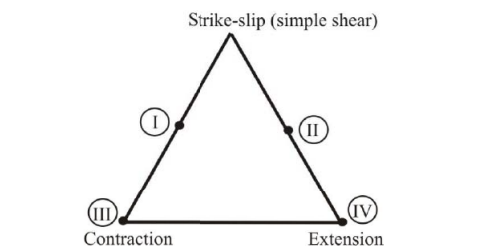
\includegraphics[width=0.5\textwidth]{figs/fig1.png}
    \caption{Image for questions 29}
    \label{fig:question29}
\end{figure}







\begin{enumerate}
\item I--pressure ridge, II--thrust, III--horst, IV--pull-apart basin
\item I--pull-apart basin, II--thrust, III--horst, IV--pressure ridge
\item I--pressure ridge, II--pull-apart basin, III--thrust, IV--horst
\item I--pull-apart basin, II--pressure ridge, III--horst, IV--thrust
\end{enumerate}


\item The best developed lineation and foliation traces in a L--S tectonite will be observed on a plane  
\begin{enumerate}
\item parallel to the lineation and foliation
\item perpendicular to the lineation and foliation
\item perpendicular to the foliation but parallel to the lineation
\item perpendicular to the lineation but parallel to the foliation
\end{enumerate}



\item Match the type of twinning (Group I) with the mineral (Group II) that best exhibits it:

\begin{multicols}{2}
\textbf{Group I}
\begin{flushleft}
P. Carlsbad\\
Q. Pericline\\
R. Brazil\\
S. Geniculated (elbow)
\end{flushleft}

\columnbreak

\textbf{Group II}
\begin{flushleft}
1. Rutile\\
2. Quartz\\
3. Orthoclase\\
4. Plagioclase
\end{flushleft}
\end{multicols}

\begin{multicols}{2}
\begin{enumerate}
\item P--3,\ Q--4,\ R--2,\ S--1
\item P--2,\ Q--4,\ R--1,\ S--3
\item P--3,\ Q--1,\ R--2,\ S--4
\item P--2,\ Q--1,\ R--3,\ S--4
\end{enumerate}
\end{multicols}


\item On inserting a first order red interference filter in SE--NW direction, the interference figure of quartz shows  
\begin{enumerate}
\item blue in NE, SW quadrants and yellow in NW, SE quadrants
\item yellow in NE, SW quadrants and blue in NW, SE quadrants
\item blue in NE, NW quadrants and yellow in SW, SE quadrants
\item yellow in NE, NW quadrants and blue in SW, SE quadrants
\end{enumerate}

\item Choose the CORRECT combination for the following two statements:  
Statement I: Four elements that make up about 90\% of the bulk Earth are Fe, O, Si and Mg (in decreasing order of wt\% abundance).  
Statement II: The four most abundant elements in the Earth's crust (in decreasing order of wt\% abundance) are O, Si, Al and Fe.  
\begin{enumerate}
\item Both Statements I and II are correct.
\item Both Statements I and II are incorrect.
\item Statement I is correct and Statement II is incorrect.
\item Statement I is incorrect and Statement II is correct.
\end{enumerate}

\item Choose the CORRECT combination for the following four statements:  
I: Anhydrous partial melting of peridotites produces basaltic magma.  
II: Hydrous melting of peridotites produces andesitic magma.  
III: Congruent melting of minerals produces liquids of compositions identical to the minerals.  
IV: Incongruent melting of minerals produces liquids of different compositions and new solids.  
\begin{multicols}{2}
\begin{enumerate}
\item All I to IV are correct.
\item I, II and III are correct but IV is incorrect.
\item I and II are correct but III and IV are incorrect.
\item All I to IV are incorrect.
\end{enumerate}
\end{multicols}

\item The value of salinity, in terms of wt.\% NaCl equivalent, of an aqueous saline bi-phase liquid--vapour fluid inclusions is determined by measurement of \_\_\_ during microthermometry.  
\begin{enumerate}
\item last ice--melting temperature
\item dissolution temperature of halite
\item eutectic temperature
\item homogenization temperature
\end{enumerate}

\item Which of the following case(s) represent(s) textural inversion in sandstone?  
Case I: Rounded grains in clayey matrix.  
Case II: Rounded, but poorly sorted grains.  
\begin{enumerate}
\item Only Case I
\item Only Case II
\item Both Case I and II
\item Neither Case I nor Case II
\end{enumerate}

\end{enumerate}

\begin{enumerate}
\setcounter{enumi}{36}

\item Which one of the following set of statements regarding the overall nature of marine shelf succession is CORRECT?  



\begin{itemize}
  \item Statement A Transgressive systems tract deposit is deepening upward.
  \item Statement B Highstand systems tract deposit is deepening upward.
  \item Statement C Falling stage systems tract deposit is deepening upward.
  \item Statement D Lowstand systems tract deposit is overall shallowing upward.
\end{itemize}

\begin{enumerate}
\item I and II
\item II and III
\item III and IV
\item I and IV
\end{enumerate}

\item Which of the following set of statements is CORRECT?  \begin{itemize}
\item Statement I: A well sorted sandstone bed showing current ripple, planar laminae, convolute laminae and prod marks. 
\item Statement II: A poorly sorted sandstone bed showing wave ripples, dish structure, pillar structure and groove casts.  
\item Statement III: A well sorted sandstone bed showing desiccation cracks, current crescent planar laminae and convolute laminae.  
\item Statement IV: A poorly sorted sandstone bed showing current ripple, planar laminae, skip marks and load casts.
\end{itemize}

\begin{multicols}{2}
\begin{enumerate}
\item I, II and III
\item II, III and IV
\item I, III and IV
\item I, II and IV
\end{enumerate}
\end{multicols}

\item In metamafites, which one of the following mineral assemblages is stable under green schist facies conditions?  
\begin{enumerate}
\item Albite + Chlorite + Actinolite + Epidote
\item Andesine + Biotite + Hornblende
\item Oligoclase + Biotite + Hornblende
\item Oligoclase + Epidote + Biotite + Hornblende
\end{enumerate}


\item Match the type of metamorphism listed in Group I with their products in Group II:

\begin{multicols}{2}
\textbf{Group I}
\begin{flushleft}
P. Contact metamorphism\\
Q. Shear zone metamorphism\\
R. Ocean floor metamorphism\\
S. Shock metamorphism
\end{flushleft}

\columnbreak

\textbf{Group II}
\begin{flushleft}
1. Impactite\\
2. Spillite\\
3. Mylonite\\
4. Skarn
\end{flushleft}
\end{multicols}

\begin{multicols}{2}
\begin{enumerate}
\item P--4,\ Q--3,\ R--2,\ S--1
\item P--2,\ Q--3,\ R--4,\ S--1
\item P--3,\ Q--1,\ R--2,\ S--4
\item P--1,\ Q--2,\ R--3,\ S--4
\end{enumerate}
\end{multicols}

\item Glaucophane schist forms in  
\begin{multicols}{2}
\begin{enumerate}
\item subduction zones
\item pull-apart basins
\item continental rifts
\item mid-oceanic ridges
\end{enumerate}
\end{multicols}

\item Which one of the following statements is CORRECT about bivalve habitat?  
\begin{enumerate}
\item Gryphaea is a burrowing variety.
\item Pholas is a free lying form.
\item Lucina is a boring variety.
\item Mytilus is a bysally attached form.
\end{enumerate}




\item Match foraminifera in Group I with its wall structure in Group II:

\begin{multicols}{2}
\textbf{Group I}
\begin{flushleft}
P. Fusulina\\
Q. Cibicides\\
R. Textularia\\
S. Quinqueloculina
\end{flushleft}

\columnbreak

\textbf{Group II}
\begin{flushleft}
1. Hyaline\\
2. Porcellaneous\\
3. Microgranular\\
4. Agglutinated
\end{flushleft}
\end{multicols}

\begin{multicols}{2}
\begin{enumerate}
\item P--1,\ Q--2,\ R--3,\ S--4
\item P--3,\ Q--2,\ R--4,\ S--1
\item P--4,\ Q--3,\ R--2,\ S--1
\item P--3,\ Q--1,\ R--4,\ S--2
\end{enumerate}
\end{multicols}



\item Which one of the following stratigraphic units represents the CORRECT order of younging?  
\begin{enumerate}
\item Trichinopally Group -- Uttatur Group -- Ariyalur Group -- Niniyur Group
\item Kopili Formation -- Sylhet Formation -- Barail Formation -- Boka Bil Formation
\item Chinji Formation -- Nagri Formation -- Dhok Pathan Formation -- Tatrot Formation
\item Barakar Formation -- Talchir Formation -- Barren Measures -- Raniganj Formation
\end{enumerate}




\item Match the Formation names in Group I with their dominant lithology in Group II:

\begin{multicols}{2}
\textbf{Group I}
\begin{flushleft}
P. Hanseran Formation\\
Q. Nagthat Formation\\
R. Bijli Formation\\
S. Shahbad Formation
\end{flushleft}

\columnbreak

\textbf{Group II}
\begin{flushleft}
1. Sandstone\\
2. Limestone\\
3. Evaporite\\
4. Volcanics
\end{flushleft}
\end{multicols}

\begin{multicols}{2}
\begin{enumerate}
\item P--3,\ Q--2,\ R--1,\ S--4
\item P--2,\ Q--1,\ R--3,\ S--4
\item P--3,\ Q--1,\ R--4,\ S--2
\item P--4,\ Q--1,\ R--2,\ S--3
\end{enumerate}
\end{multicols}


\item Match the economic deposits in Group I with their occurrence in stratigraphic units in Group II:

\begin{multicols}{2}
\textbf{Group I}
\begin{flushleft}
P. Phosphate\\
Q. Manganese\\
R. Chromite\\
S. Barite
\end{flushleft}

\columnbreak

\textbf{Group II}
\begin{flushleft}
1. Sargur Group\\
2. Nallamalai Group\\
3. Udaipur Formation\\
4. Mansar Formation
\end{flushleft}
\end{multicols}

\begin{multicols}{2}
\begin{enumerate}
\item P--1,\ Q--3,\ R--4,\ S--2
\item P--3,\ Q--4,\ R--2,\ S--1
\item P--2,\ Q--1,\ R--4,\ S--3
\item P--3,\ Q--4,\ R--1,\ S--2
\end{enumerate}
\end{multicols}



\item Match the basin type in Group I with Indian example in Group II:

\begin{multicols}{2}
\textbf{Group I}
\begin{flushleft}
P. Foreland basin\\
Q. Passive margin\\
R. Fore-arc\\
S. Failed rift
\end{flushleft}

\columnbreak

\textbf{Group II}
\begin{flushleft}
1. Kerala--Konkan\\
2. Cambay\\
3. Ganga\\
4. Andaman
\end{flushleft}
\end{multicols}

\begin{multicols}{2}
\begin{enumerate}
\item P--3,\ Q--2,\ R--4,\ S--1
\item P--3,\ Q--1,\ R--4,\ S--2
\item P--4,\ Q--1,\ R--3,\ S--2
\item P--1,\ Q--2,\ R--4,\ S--3
\end{enumerate}
\end{multicols}




\item Choose the CORRECT set of statements.  
Statement I: The hydrocarbon source rock in Cambay basin is of Jurassic age.  
Statement II: Borholla field is in Assam basin.  
Statement III: Toulene is an aromatic hydrocarbon.  
Statement IV: Porosity of a reservoir rock increases with increase in sorting.  
\begin{multicols}{2}
\begin{enumerate}
\item I, II and III
\item II, III and IV
\item I and IV
\item I and III only
\end{enumerate}
\end{multicols}

\item The figure given below represents a scattered Band 5 of a satellite imagery. The fields rectangular boxes along with their class n point P by Minimum Distance to Mean (M
are

\begin{figure}[H]
    \centering
    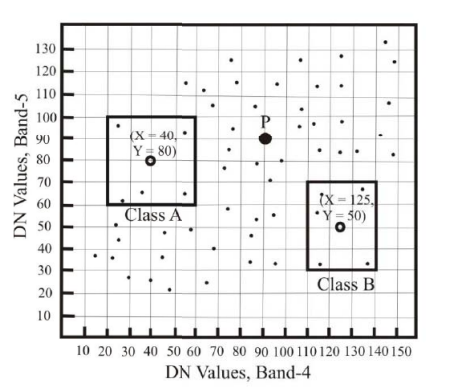
\includegraphics[width=0.4\textwidth]{figs/fig2.png}
    \caption{Image for questions 49}
    \label{fig:question49}
\end{figure}

\begin{enumerate}
\item Class A by MDM and Class B by NN
\item Class A by NN and Class B by MDM
\item Class A by both MDM and NN
\item Class B by both MDM and NN
\end{enumerate}

\item The hydraulic head at the contact (X--Y) is \_\_\_ m. (round off to 2 decimal places).  
\vspace{0.5cm}

\item The Concavity Index of the river is \_\_\_ \%.  
\vspace{0.5cm}

\begin{figure}[H]
    \centering
    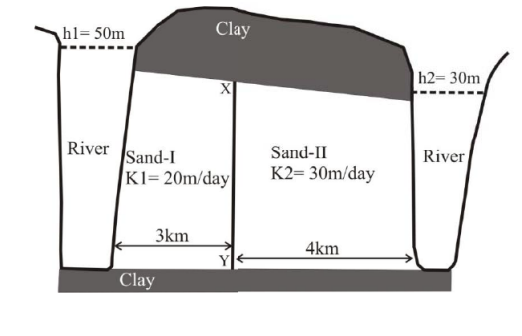
\includegraphics[width=0.6\textwidth]{figs/fig3.png}
    \caption{Image for questions 50}
    \label{fig:question50}
\end{figure}




\item For producing 1 kg of gold from an ore having an assay of 2 ppm Au, \_\_\_ $\times 10^3$ kg of ore needs to be processed.  
\vspace{0.5cm}

\item The uncorrected point load strength index is \_\_\_ MPa.  
\vspace{0.5cm}
\end{enumerate}
\begin{enumerate}
\setcounter{enumi}{53}

\item A hypothetical garnet peridotite composed of 60\% olivine, 25\% orthopyroxene, 10\% clinopyroxene and 5\% garnet undergoes 10\% batch melting described by  
$C_L = \dfrac{C_0}{F + D - F \cdot D}$  
where $F$ is the degree of melting and $D$ is the bulk partition coefficient.  
The ratio of Ce in the melt to the original rock will be \_\_\_. (round off to 2 decimal places).  
(The $K_D$ values of Ce for olivine, orthopyroxene, clinopyroxene and garnet are 0.001, 0.003, 0.10 and 0.02, respectively.)  
\vspace{0.5cm}

\item $^{87}$Rb decays to $^{87}$Sr with a decay constant $\lambda = 1.42 \times 10^{-11}$ per year. If at the time of formation, a system contains $8 \times 10^{4}$ atoms of $^{87}$Rb and $10^{3}$ atoms of $^{87}$Sr, the number of $^{87}$Sr atoms in this system at the end of 4 half--lives will be \_\_\_ $\times 10^{3}$.  
Assume closed system evolution for the parent--daughter pair.  
\vspace{0.5cm}

\item The Young's modulus $E$ is related to the Lamé parameter $\lambda$ for a Poisson solid as:  
\begin{multicols}{4}
\begin{enumerate}
\item $E = 2.5\,\lambda$
\item $E = 1.5\,\lambda$
\item $E = 2\,\lambda$
\item $E = 0.5\,\lambda$
\end{enumerate}
\end{multicols}

\end{enumerate}

\begin{enumerate}
\setcounter{enumi}{56}

\item Which one of the following seismic phases is the earliest arrival in the P shadow zone?
\begin{multicols}{4}
\begin{enumerate}
\item PKiKP
\item PPP
\item Pdiff
\item PKIKP
\end{enumerate}
\end{multicols}

\item A reversed refraction survey was done over a two layered medium with the interface between them dipping at an angle of 15$^\circ$. The velocities in the upper and lower medium are $V_1$ and $V_2$ respectively, with $V_2 > V_1$. If the critical angle is 45$^\circ$, then which one of the following is CORRECT? (Vu and Va are updip and downdip velocities).
\begin{multicols}{4}
\begin{enumerate}
\item $V_1 = V_a = V_u$
\item $V_u > V_a > V_1$
\item $V_1 > V_a < V_u$
\item $V_u < V_a > V_1$
\end{enumerate}
\end{multicols}

\item In a migrated seismic time section:
\begin{enumerate}
\item both synclines and anticlines appear tighter
\item both synclines and anticlines appear broader
\item synclines appear tighter and anticlines appear broader
\item synclines appear broader and anticlines appear tighter
\end{enumerate}

\item Which one of the following is \textbf{CORRECT} for the density porosity ($\phi_D$) and neutron porosity ($\phi_N$) estimated for a finely interbedded organic--rich, shaly sandstone formation relative to those for a shale--free  sandstone formation at shallow depths?



\begin{enumerate}
\item $\phi_N$ decreases and $\phi_D$ increases
\item $\phi_N$ increases and $\phi_D$ decreases
\item both $\phi_N$ and $\phi_D$ decrease
\item both $\phi_N$ and $\phi_D$ increase
\end{enumerate}

\item Which one of the following statements is INCORRECT with regard to Nuclear Magnetic Resonance (NMR) logging? ($\phi_{\mathrm{NMR}}$ -- NMR derived total porosity, $\phi_D$ -- Density porosity)
\begin{enumerate}
\item The relaxation time ($T_2$) decreases with decrease in pore size.
\item $\phi_{\mathrm{NMR}}$ is greater than $\phi_D$ in a water saturated sandstone formation.
\item NMR logs provide lithology--independent measurement of total porosity.
\item $\phi_{\mathrm{NMR}}$ is less than $\phi_D$ in a gas saturated shaly sandstone formation.
\end{enumerate}

\item A 3--D seismic tomography experiment was carried out with an  interstation spacing of $X\,\mathrm{km}$. The subsurface velocity perturbations  in three--dimensional blocks were estimated with block sizes of $2X\,\mathrm{km}$  and $0.5X\,\mathrm{km}$ in case~1 and case~2, respectively. Which one of the 
following statements is \textbf{CORRECT}?


\begin{enumerate}
\item Spatial resolution is poor and variance is small for case 1.
\item Spatial resolution is good and variance is small for case 2.
\item Spatial resolution is good and variance is large for case 1.
\item Spatial resolution is poor and variance is large for case 2.
\end{enumerate}

\item A shallow--focus, great earthquake with a seismic moment of  $2.5 \times 10^{40}\ \mathrm{dyne\! \cdot\! cm}$ is recorded at an epicentral  distance of $50^{\circ}$. The body--wave magnitude ($m_b$),  surface--wave magnitude ($M_s$), and moment magnitude ($M_w$) were  estimated. Which one of the following is \textbf{CORRECT}is

\begin{enumerate}
\item $m_b > M_s > M_w$
\item $m_b = M_s = M_w$
\item $m_b < M_s < M_w$
\item $m_b < M_s > M_w$
\end{enumerate}

\item A pair of current electrodes C$_1$ ($+I$) and C$_2$ ($-I$) is placed $50\,\mathrm{m}$ apart over a homogeneous structure of resistivity $100\,\Omega\ \mathrm{m}$. A current of $1\,\mathrm{A}$ flows through the subsurface. Which one of the following is \textbf{CORRECT} for the potential ($V_p$) and the horizontal component of electric field ($E_x$) at a point $P$ located exactly below the midpoint between C$_1$ and C$_2$ at a depth of $10\,\mathrm{m}$?

\begin{figure}[H]
    \centering
    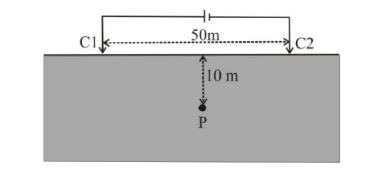
\includegraphics[width=0.4\textwidth]{figs/fig5.png}
    \caption{Image for questions 64}
    \label{fig:question64}
\end{figure}

\begin{multicols}{2}
\begin{enumerate}
\item $V_p = 0$ and $E_x = 0$
\item $V_p = 0$ and $E_x \neq 0$
\item $V_p \neq 0$ and $E_x = 0$
\item $V_p \neq 0$ and $E_x \neq 0$
\end{enumerate}
\end{multicols}

\item A massive sulphide body in the subsurface is partially above the water table. According to the pH variation hypothesis for the origin of Self Potential, which one of the following statements is CORRECT for such a body?
\begin{enumerate}
\item Acidic above and basic below the water table
\item Basic above and acidic below the water table
\item Acidic above and below the water table
\item Basic above and below the water table
\end{enumerate}


\item The phase difference between the input and output signals for a ``Compensator device'' used in electromagnetic prospecting to nullify the effect of the primary field at the receiver coil is:
\begin{multicols}{4}
\begin{enumerate}
\item 0$^\circ$
\item 45$^\circ$
\item 90$^\circ$
\item 180$^\circ$
\end{enumerate}
\end{multicols}

\item In an electromagnetic scale modeling experiment in the lab, the relation between the field and lab geometrical scaling factor ($n$) with the field and lab resistivity ($\rho_f$ \& $\rho_m$) as well as frequencies ($f_f$ \& $f_m$) will be (subscripts f and m refer to field and lab systems and $n \gg 1$):
\begin{multicols}{2}
\begin{enumerate}
\item $n^2 = \dfrac{\rho_f f_f}{\rho_m f_m}$
\item $n^2 = \dfrac{\rho_f f_m}{\rho_m f_f}$
\item $n^2 = \dfrac{\rho_m f_m}{\rho_f f_f}$
\item $n^2 = \dfrac{\rho_m f_f}{\rho_f f_m}$
\end{enumerate}
\end{multicols}

\item If $G(\omega)$ is the Fourier transform of $g(t)$, then the Fourier transform of $g(t + \ln 2)$ will be:
\begin{multicols}{2}
\begin{enumerate}
\item $e^{-2j\omega} G(\omega)$
\item $e^{2j\omega} G(\omega)$
\item $2e^{j\omega} G(\omega)$
\item $2e^{-j\omega} G(\omega)$
\end{enumerate}
\end{multicols}

\item The primary objective of ``Regularization'' in geophysical inversion is to:

\begin{multicols}{4}
\begin{enumerate}
\item improve the resolution  
\item reduce the non--uniqueness  
\item enhance the condition number  
\item stabilize the inversion process  
\end{enumerate}
\end{multicols}




\item Let $P$ be a point on the Earth's surface defined by radius $r$, colatitude $\theta$, 
and longitude $\phi$ in a spherical coordinate system. The three components of the magnetic 
induction $\mathbf{B}$ at $P$ in the Cartesian coordinate system are $B_x$, $B_y$, and $B_z$ 
(x--North, y--East, z--downward). For the relation $\mathbf{B} = -\nabla V$ 
(where $V$ is the magnetic potential), the quantities $B_x$, $B_y$, and $B_z$ can be expressed 
in spherical coordinates as:
\vspace{0.5cm}


\begin{enumerate}
    \item $B_x = \frac{\partial V}{\partial \theta}, \quad 
          B_y = \frac{1}{\sin\theta}\,\frac{\partial V}{\partial \phi}, \quad
          B_z = \frac{\partial V}{\partial r}$
          
    \item $B_x = -\frac{\partial V}{\partial \theta}, \quad 
          B_y = -\frac{1}{\sin\theta}\,\frac{\partial V}{\partial \phi}, \quad
          B_z = -\frac{\partial V}{\partial r}$
          
    \item $B_x = -\frac{\partial V}{\partial \theta}, \quad 
          B_y = -\frac{1}{\sin\theta}\,\frac{\partial V}{\partial \phi}, \quad
          B_z = \frac{\partial V}{\partial r}$
          
    \item $B_x = \frac{\partial V}{\partial \theta}, \quad 
          B_y = \frac{1}{\sin\theta}\,\frac{\partial V}{\partial \phi}, \quad
          B_z = -\frac{\partial V}{\partial r}$
\end{enumerate}
\vspace{0.5cm}


\item In gravity anomalies, the \textquotedblleft Indirect effect\textquotedblright\ mainly arises from:
\begin{enumerate}
\item sources outside the area of investigation
\item improper instrument drift
\item effect of mass lying between the geoid and ellipsoid
\item short--wavelength uncompensated masses in the subsurface
\end{enumerate}

\item For defining the axial geocentric magnetic dipole of the Earth's magnetic field using the spherical harmonic expression for magnetic potential, the three non--zero Gauss coefficients for $n = 1$ are
\begin{multicols}{2}
\begin{enumerate}
\item $g_1^0, g_1^2, h_1^0$
\item $g_1^2, g_1^1, h_1^1$
\item $g_1^1, g_1^0, h_1^2$
\item $g_1^2, g_1^1, h_1^0$
\end{enumerate}
\end{multicols}

\item The flexural rigidity ($D$) of the oceanic lithosphere (assuming no secondary thermal 
perturbations):
\begin{enumerate}
\item increases with both age and plate cooling
\item decreases with age and increases with plate cooling
\item increases with age and decreases with plate thickness
\item decreases with both age and plate thickness
\end{enumerate}
\vspace{0.5cm}

\item If $\Delta J$ and $\Delta \rho$ are the uniform magnetization and density contrasts of a point 
source, the relation between the vertical components of the gravity ($g_z$) and magnetic ($T_z$) 
anomalies can be expressed (neglecting long--wavelength components) as (where $G$ is the gravitational constant):
\begin{enumerate}
\item $T_z = G\,\Delta J \, \partial g_z \, \Delta\epsilon \, \theta_\alpha$
\item $T_z = G\,\Delta J \, \partial g_z \, 2\pi\,\Delta\sigma \, \theta_\epsilon$
\item $T_z = \frac{\Delta J}{G\,\Delta\rho}\,\partial g_z$
\item $T_z = \frac{\Delta\rho}{G\,\Delta J}\,\partial g_z$
\end{enumerate}
\vspace{0.5cm}

\item Which one of the following statements about the gravity anomalies on land is CORRECT?
\vspace{0.5cm}
\item Free--air and Bouguer anomalies are always positively correlated with elevation.
\vspace{0.5cm}

\item Isostatic anomalies are not useful to understand the crustal heterogeneities.
\vspace{0.5cm}

\item Vertical derivatives are used to enhance the gravity effects of deep--seated bodies.
\vspace{0.5cm}

\item $X$--horizontal gradient ($\partial/\partial x$) maps enhance/sharpen anomalies of bodies trending N--S ($X$--East, $Y$--North, $Z$--downward).
\vspace{0.5cm}



\item An aeromagnetic survey is conducted over an area with outcropping magnetic sources. The 
aircraft is flying at a height of $250\,\mathrm{m}$ with a speed of $200\,\mathrm{km/hr}$. In order to fully 
define the magnetic anomalies along the flight path, the largest sampling interval (Proton 
Precession Magnetometer) will be \underline{\hspace{10mm}} seconds.
\vspace{0.5cm}

\item In an abandoned mine--site, three hollow spherical cavities are located below the surface, centered at depths of $50$, $100$, and $150\,\mathrm{m}$. Assuming each produces $\sim 0.05\,\mathrm{mGal}$ and do not interfere, the most ideal (largest) grid spacing to correctly delineate these cavities is \underline{\hspace{10mm}} metres.
\vspace{0.5cm}

\item A split--spread reflection survey is carried out along a profile in the direction of a dipping  interface. The difference in arrival times of the reflected waves from the interface at two  geophones with an offset of $1000\,\mathrm{m}$ on both sides is $20\,\mathrm{ms}$. If the velocity of the upper 
layer is $3000\,\mathrm{m/s}$, then the dip of the bed is \underline{\hspace{10mm}} degrees.
\vspace{0.5cm}

\item The bulk resistivity of a carbonate formation having $10\%$ porosity and $75\%$ hydrocarbon 
saturation is $500\,\Omega\ \mathrm{m}$. The bulk resistivity of the formation when the porosity is doubled 
and saturation is $100\%$ water is \underline{\hspace{10mm}} $\Omega\ \mathrm{m}$.
\vspace{0.5cm}

\item In a seismogram of a shallow--focus ($h = 5\,\mathrm{km}$) earthquake, the 
$S$--$P$ time difference is $1.34\,\mathrm{s}$. Given $V_{P} = 6.0\,\mathrm{km\,s^{-1}}$ 
and $\nu = 0.27$, the epicentral distance is \underline{\hspace{10mm}}~km
\vspace{0.5cm}

\item A two--electrode array is placed over a vertical contact (strike perpendicular to page). If $1\,\mathrm{A}$ 
current flows, the potential at electrode $P_1$ will be \underline{\hspace{10mm}} mV.  
(Resistivities: $\rho_1=100\,\Omega\mathrm{m}$, $\rho_2=200\,\Omega\mathrm{m}$; $C_2$ and $P_2$ at infinity.)

\begin{figure}[H]
    \centering
    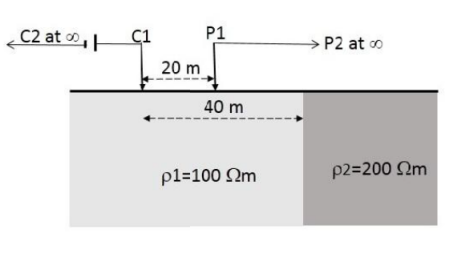
\includegraphics[width=0.4\textwidth]{figs/fig6.png}
    \caption{Image for questions 81}
    \label{fig:question81}
\end{figure}
\vspace{0.5cm}

\item In an electrical resistivity imaging survey, an Axial Dipole--dipole array is placed with centre--centre 
distance $100\,\mathrm{m}$. Dipole length $10\,\mathrm{m}$. If $5\,\mathrm{A}$ current and $50\,\mathrm{mV}$ potential difference 
are measured, the apparent resistivity is \underline{\hspace{10mm}} $\Omega\ \mathrm{m}$.
\vspace{0.5cm}

\item In an EM land survey, the resultant field at point $P$ makes a $60^\circ$ angle from vertical.  
A $30\,\mathrm{mV}$ signal is observed with a horizontal coil. The magnitude when the coil is perpendicular 
to the resultant field is \underline{\hspace{10mm}} mV.
\vspace{0.5cm}

\item A vibroseis source sweeps $10$--$100\,\mathrm{Hz}$. The maximum sampling interval to recover the signal 
is \underline{\hspace{10mm}} milliseconds.
\vspace{0.5cm}

\item The abundance of $^{234}\mathrm{U}$ in secular equilibrium with parent $^{238}\mathrm{U}$ will be 
\underline{\hspace{10mm}} $\times 10^{-3}\ \%$.  
($T_{1/2}$: $^{238}\mathrm{U} = 4.467\times 10^9\,$y; $^{234}\mathrm{U} = 2.44\times 10^5\,$y; abundance of $^{238}\mathrm{U} = 99.28\%$)
\vspace{0.5cm}



\end{enumerate}











































































































































\end{document}